\keepXColumns
\section{Analisi dei requisiti}
\label{analisi-requisiti}
La fase di \textbf{analisi dei requisiti} consiste nello studio e nell'esame delle esigenze espresse dall'azienda, con l'obiettivo di definire in modo preciso e completo i requisiti del sistema.  
Questa parte del progetto si è svolta nell'arco di due settimane, durante le quali ho organizzato incontri regolari con il tutor aziendale per confrontarsi su progressi, criticità e possibili soluzioni. Le principali attività condotte includono:
\begin{itemize}
    \item \textbf{Sessioni di \textit{brainstorming}} con il tutor, finalizzate alla definizione degli obiettivi e delle priorità del sistema;
    \item \textbf{Studio della documentazione} di sistemi \textit{honeypot} esistenti, per comprendere metodologie consolidate e funzionalità tipiche;
    \item \textbf{Analisi delle \textit{best practice}} in ambito \textit{cybersecurity} per sistemi \textit{ETL}, a garanzia di sicurezza e affidabilità;
    \item \textbf{Valutazione dei vincoli tecnologici} imposti dall'ambiente aziendale, tra cui piattaforme disponibili, linguaggi di programmazione e strumenti di monitoraggio.
\end{itemize}
Dall'analisi effettuata sono emersi i \hyperref[casi-uso]{casi d'uso} sulla quale si è basato il progetto.
\subsection{Casi d'uso}
\label{casi-uso}
I \textbf{casi d'uso} descrivono una funzionalità specifica che il sistema deve fornire a uno o più attori (che possono essere utenti o altri sistemi), indicando le interazioni e i risultati ottenuti dal punto di vista degli attori.
Per sviluppare i casi d'uso abbiamo utilizzato il linguaggio \gls{uml}\glsadd{uml_def}, uno strumento di modellazione che mostra le interazioni tra attori e casi d'uso attraverso relazioni come \textit{<<include>>}, \textit{<<extend>>} e generalizzazioni.
La seguente convenzione di nomenclatura supporta l'identificazione dei casi d'uso e ne facilita l'organizzazione e la tracciabilità:\\
\begin{center}
\textbf{UC.ID.subID}
\end{center}
\begin{itemize}
    \item \textbf{UC}: è l'identificatore dei casi d'uso;
    \item \textbf{ID}: è l'identificatore numerico del caso d'uso principale;
    \item \textbf{subID}: è l'identificatore numerico dei sotto-casi d'uso che specifica i casi d'uso associati a un caso d'uso principale.
\end{itemize}
\begin{figure}[H]
    \begin{center}
        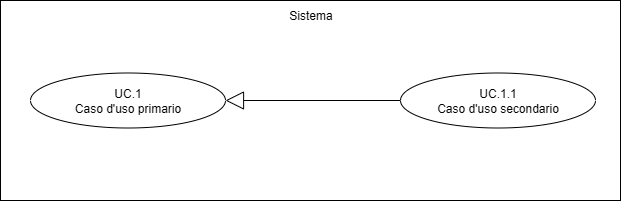
\includegraphics[alt={Esempio di caso d'uso e sotto-caso d'uso}, width=0.8\columnwidth]{img/esempio_uc.png}
        \caption{Esempio di caso d'uso e sotto-caso d'uso.}
        \label{fig:es-uc}
    \end{center}
\end{figure}
\subsection*{Attori dei casi d'uso}
Nel contesto dei casi d'uso, gli attori del sistema si suddividono in due categorie principali: \textbf{attori primari} e \textbf{attori secondari}.\\\\
Gli \textbf{attori primari} sono coloro che avviano attivamente un caso d'uso con l'obiettivo di ottenere un risultato specifico attraverso l'interazione diretta con il sistema. Rappresentano gli utenti o le entità che traggono un beneficio concreto dall'esecuzione del caso d'uso.\\
All'interno del progetto l'attore principale è:
\begin{itemize}
    \item \textbf{Utente}: cioè un utente membro del \textit{team} di \textit{cybersecurity} che ha accesso all'\textit{honeypot}.
\end{itemize}
Al contrario, gli \textbf{attori secondari} non iniziano il caso d'uso, ma forniscono supporto o servizi necessari affinché il sistema possa completarlo correttamente. Interagiscono in modo indiretto o passivo, contribuendo al funzionamento del processo senza esserne i promotori principali. In questo caso all'interno del sistema non sono presenti attori secondari, poiché non ci sono entità che svolgono un ruolo di supporto indiretto al processo.\\
\begin{figure}[H]
    \begin{center}
        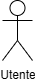
\includegraphics[alt={Esempio di attore}, width=0.075\columnwidth]{img/attore.png}
        \caption{Esempio di attore.}
        \label{fig:es-attore}
    \end{center}
\end{figure}
\subsubsection*{Lista dei casi d'uso}
Di seguito si trovano i casi d'uso principali del sistema.
Non sono riportati tutti i casi d'uso individuati in fase di analisi, ma soltanto quelli ritenuti maggiormente rappresentativi e funzionali alla comprensione delle caratteristiche essenziali del sistema.
La scelta di limitarne il numero risponde a due esigenze: da un lato evitare ridondanze o descrizioni eccessivamente dettagliate di funzionalità marginali, dall'altro garantire una visione chiara e sintetica delle capacità chiave del sistema in relazione ai suoi obiettivi progettuali.
\begin{center}
\begin{longtable}{|p{0.3\textwidth}|p{0.65\textwidth}|}
\hline
\multicolumn{2}{|c|}{\textbf{UC.1}}\\ 
\hline 
\endfirsthead
\multicolumn{2}{c}{{\bfseries \tablename\ \thetable{} -- Continuo della tabella}}\\
\hline
\multicolumn{2}{|c|}{\textbf{UC.1}}\\ \hline 
\endhead
\hline
\multicolumn{2}{|r|}{{Continua nella prossima pagina...}}\\
\hline
\endfoot
\endlastfoot
% Riga immagine che occupa entrambe le colonne
\multicolumn{2}{|c|}{
    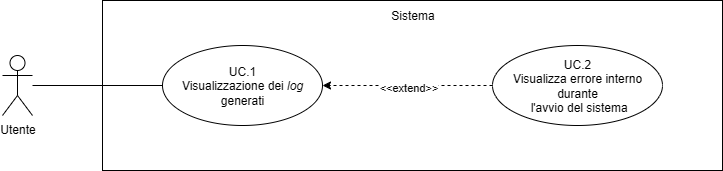
\includegraphics[width=\textwidth]{img/UC-1.png}
}\\ \hline
\textbf{Pre-condizioni} & Il sistema è attivo e funzionante. \\ \hline
\textbf{Post-condizioni} & Vengono visualizzati i \textit{log} generati dal sistema \textit{honeypot}. \\ \hline
\textbf{Attori principali} & Utente \\ \hline
\textbf{Scenario principale} & 
\begin{itemize}
    \item L'utente richiede la visualizzazione dei \textit{log} del sistema;
    \item Il sistema verifica la presenza e la conformità dei \textit{log};
    \item I dati del sistema vengono visualizzati in ordine cronologico di creazione.
\end{itemize} \\ \hline
\textbf{Scenario secondario} & 
\begin{itemize}
    \item Si verifica un errore interno durante l'avvio del sistema che impedisce la visualizzazione dei \textit{log} (\hyperref[tab:uc-2]{UC.2}).
\end{itemize} \\ \hline
\caption{Diagramma del caso d'uso UC.1 - Visualizzare i \textit{log} del sistema \textit{honeypot}.}
\label{tab:uc-1}
\end{longtable}
\end{center}

\begin{center}
\begin{longtable}{|p{0.3\textwidth}|p{0.65\textwidth}|}
\hline
\multicolumn{2}{|c|}{\textbf{UC.2}}\\ 
\hline 
\endfirsthead
\multicolumn{2}{c}{{\bfseries \tablename\ \thetable{} -- Continuo della tabella}}\\
\hline
\multicolumn{2}{|c|}{\textbf{UC.2}}\\ \hline 
\endhead
\hline
\multicolumn{2}{|r|}{{Continua nella prossima pagina...}}\\
\hline
\endfoot
\endlastfoot
% Riga immagine che occupa entrambe le colonne
\textbf{Pre-condizioni} & L'avvio delle diverse componenti del sistema non avviene correttamente. \\ \hline
\textbf{Post-condizioni} & L'utente visualizza gli errori che impediscono l'avvio del sistema e il loro livello di gravità. \\ \hline
\textbf{Attori principali} & Utente \\ \hline
\textbf{Scenario principale} & 
\begin{itemize}
    \item L'utente avvia il sistema;
    \item Il sistema verifica lo stato delle sue componenti;
    \item Se si verifica un errore, il sistema comunica all'utente quale componente non si è avviata correttamente.
\end{itemize} \\ \hline
\textbf{Scenario secondario} & 
\begin{itemize}
    \item N/A 
\end{itemize} \\ \hline
\caption{Diagramma del caso d'uso UC.2 - Visualizza errore interno durante l'avvio del sistema.}
\label{tab:uc-2}
\end{longtable}
\end{center}

\begin{center}
\begin{longtable}{|p{0.3\textwidth}|p{0.65\textwidth}|}
\hline
\multicolumn{2}{|c|}{\textbf{UC.3}}\\ 
\hline 
\endfirsthead
\multicolumn{2}{c}{{\bfseries \tablename\ \thetable{} -- Continuo della tabella}}\\
\hline
\multicolumn{2}{|c|}{\textbf{UC.3}}\\ \hline 
\endhead
\hline
\multicolumn{2}{|r|}{{Continua nella prossima pagina...}}\\
\hline
\endfoot
\endlastfoot
% Riga immagine che occupa entrambe le colonne
\multicolumn{2}{|c|}{
    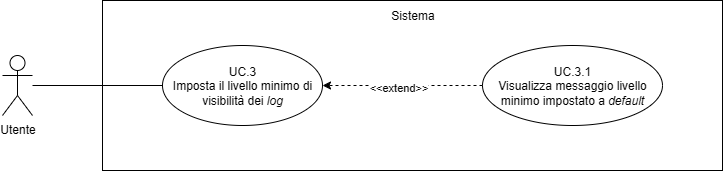
\includegraphics[width=\textwidth]{img/UC-3.png}
}\\ \hline
\textbf{Pre-condizioni} & Il sistema è in fase di avvio. \\ \hline
\textbf{Post-condizioni} & Il livello minimo dei \textit{log} da visualizzare è impostato. \\ \hline
\textbf{Attori principali} & Utente \\ \hline
\textbf{Scenario principale} & 
\begin{itemize}
    \item L'utente visualizza i possibili livelli minimi del sistema;
    \item L'utente seleziona il livello minimo desiderato;
    \item Il sistema applica la nuova configurazione e conferma l'avvenuta modifica.
\end{itemize} \\ \hline
\textbf{Scenario secondario} & 
\begin{itemize}
    \item L'utente seleziona un livello non valido, oppure non seleziona nessun livello.
\end{itemize} \\ \hline
\caption{Diagramma del caso d'uso UC.3 - Impostare il livello minimo dei \textit{log} da visualizzare.}
\label{tab:uc-3}
\end{longtable}
\end{center}

\begin{center}
\begin{longtable}{|p{0.3\textwidth}|p{0.65\textwidth}|}
\hline
\multicolumn{2}{|c|}{\textbf{UC.4}}\\ 
\hline 
\endfirsthead
\multicolumn{2}{c}{{\bfseries \tablename\ \thetable{} -- Continuo della tabella}}\\
\hline
\multicolumn{2}{|c|}{\textbf{UC.4}}\\ \hline 
\endhead
\hline
\multicolumn{2}{|r|}{{Continua nella prossima pagina...}}\\
\hline
\endfoot
\endlastfoot
% Riga immagine che occupa entrambe le colonne
\multicolumn{2}{|c|}{
    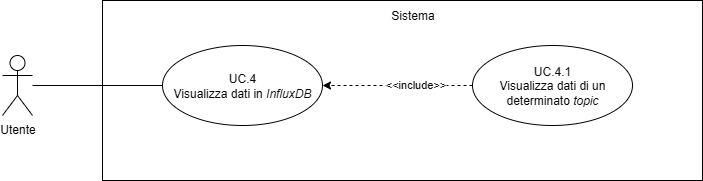
\includegraphics[width=\textwidth]{img/UC-4.png}
}\\ \hline
\textbf{Pre-condizioni} & Il sistema è attivo e funzionante. \\ \hline
\textbf{Post-condizioni} & Vengono visualizzati i dati presenti in \textit{InfluxDB}. \\ \hline
\textbf{Attori principali} & Utente \\ \hline
\textbf{Scenario principale} & 
\begin{itemize}
    \item L'utente richiede la visualizzazione dei dati presenti in \textit{InfluxDB};
    \item Il sistema verifica la presenza e la conformità dei dati;
    \item I dati presenti in \textit{InfluxDB} vengono visualizzati in base ai filtri selezionati.
\end{itemize} \\ \hline
\textbf{Scenario secondario} & 
\begin{itemize}
    \item Non sono presenti dati in \textit{InfluxDB} da visualizzare;
    \item Il sistema non mostra alcun dato all'utente.
\end{itemize} \\ \hline
\caption{Diagramma del caso d'uso UC.4 - Visualizzare i dati presenti in \textit{InfluxDB}.}
\label{tab:uc-4}
\end{longtable}
\end{center}

\begin{center}
\begin{longtable}{|p{0.3\textwidth}|p{0.65\textwidth}|}
\hline
\multicolumn{2}{|c|}{\textbf{UC.5}}\\ 
\hline 
\endfirsthead
\multicolumn{2}{c}{{\bfseries \tablename\ \thetable{} -- Continuo della tabella}}\\
\hline
\multicolumn{2}{|c|}{\textbf{UC.5}}\\ \hline 
\endhead
\hline
\multicolumn{2}{|r|}{{Continua nella prossima pagina...}}\\
\hline
\endfoot
\endlastfoot
% Riga immagine che occupa entrambe le colonne
\multicolumn{2}{|c|}{
    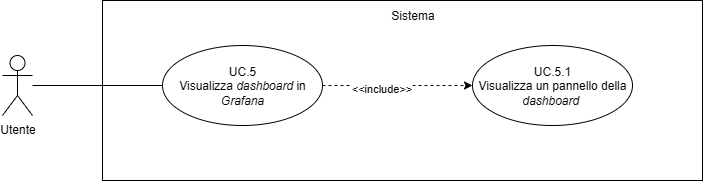
\includegraphics[width=\textwidth]{img/UC-5.png}
}\\ \hline
\textbf{Pre-condizioni} & Il sistema è attivo e funzionante. \\ \hline
\textbf{Post-condizioni} & Viene visualizzata una \textit{dashboard} in \textit{Grafana}. \\ \hline
\textbf{Attori principali} & Utente \\ \hline
\textbf{Scenario principale} & 
\begin{itemize}
    \item L'utente richiede la visualizzazione di una \textit{dashboard} in \textit{Grafana};
    \item Il sistema verifica la presenza e la conformità della \textit{dashboard};
    \item La \textit{dashboard} viene visualizzata con i dati aggiornati in tempo reale.
\end{itemize} \\ \hline
\textbf{Scenario secondario} & 
\begin{itemize}
    \item Non sono presenti dati in \textit{InfluxDB} da visualizzare;
    \item Il sistema non mostra alcun dato all'utente.
\end{itemize} \\ \hline
\caption{Diagramma del caso d'uso UC.5 - Visualizzare una \textit{dashboard} in \textit{Grafana}.}
\label{tab:uc-5}
\end{longtable}
\end{center}

\begin{center}
\begin{longtable}{|p{0.3\textwidth}|p{0.65\textwidth}|}
\hline
\multicolumn{2}{|c|}{\textbf{UC.6}}\\ 
\hline 
\endfirsthead
\multicolumn{2}{c}{{\bfseries \tablename\ \thetable{} -- Continuo della tabella}}\\
\hline
\multicolumn{2}{|c|}{\textbf{UC.6}}\\ \hline 
\endhead
\hline
\multicolumn{2}{|r|}{{Continua nella prossima pagina...}}\\
\hline
\endfoot
\endlastfoot
% Riga immagine che occupa entrambe le colonne
\multicolumn{2}{|c|}{
    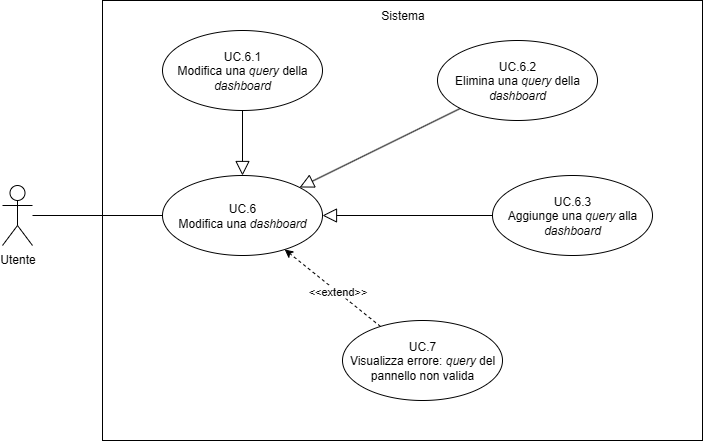
\includegraphics[width=\textwidth]{img/UC-6.png}
}\\ \hline
\textbf{Pre-condizioni} & Il sistema è attivo e funzionante. \\ \hline
\textbf{Post-condizioni} & Viene modificata una \textit{dashboard} in \textit{Grafana}. \\ \hline
\textbf{Attori principali} & Utente \\ \hline
\textbf{Scenario principale} & 
\begin{itemize}
    \item L'utente modifica una \textit{dashboard} in \textit{Grafana};
    \item Il sistema verifica la conformità della \textit{query};
    \item La \textit{dashboard} viene aggiornata con le nuove impostazioni.
\end{itemize} \\ \hline
\textbf{Scenario secondario} & 
\begin{itemize}
    \item La modifica non è conforme agli standard di \textit{Grafana} (\hyperref[tab:uc-7]{UC.7}).
\end{itemize} \\ \hline
\caption{Diagramma del caso d'uso UC.6 - Modificare una \textit{dashboard} in \textit{Grafana}.}
\label{tab:uc-6}
\end{longtable}
\end{center}

\begin{center}
\begin{longtable}{|p{0.3\textwidth}|p{0.65\textwidth}|}
\hline
\multicolumn{2}{|c|}{\textbf{UC.7}}\\ 
\hline 
\endfirsthead
\multicolumn{2}{c}{{\bfseries \tablename\ \thetable{} -- Continuo della tabella}}\\
\hline
\multicolumn{2}{|c|}{\textbf{UC.7}}\\ \hline 
\endhead
\hline
\multicolumn{2}{|r|}{{Continua nella prossima pagina...}}\\
\hline
\endfoot
\endlastfoot
\textbf{Pre-condizioni} & La modifica effettuata dall'utente non è valida. \\ \hline
\textbf{Post-condizioni} & Viene visualizzato il pannello di errore. \\ \hline
\textbf{Attori principali} & Utente \\ \hline
\textbf{Scenario principale} & 
\begin{itemize}
    \item L'utente modifica una \textit{dashboard} in \textit{Grafana};
    \item Il sistema verifica la conformità della modifica effettuata;
    \item La modifica non è conforme agli standard di \textit{Grafana};
    \item Il sistema visualizza il pannello di errore.
\end{itemize} \\ \hline
\textbf{Scenario secondario} & 
\begin{itemize}
    \item N/A
\end{itemize} \\ \hline
\caption{Diagramma del caso d'uso UC.7 - Visualizza errore: \textit{query} del pannello non valida.}
\label{tab:uc-7}
\end{longtable}
\end{center}
\subsection{Requisiti}
\label{requisiti}
I requisiti si dividono in tre categorie principali: funzionali, non funzionali e di vincolo, che specificano rispettivamente cosa deve fare il sistema, come deve funzionare e quali condizioni deve rispettare per operare. 
I primi sono le azioni che il sistema deve compiere, mentre i secondi sono le qualità che deve avere (come la velocità o la sicurezza). 
I requisiti di vincolo, invece, riguardano le restrizioni imposte al sistema, come la piattaforma su cui deve girare o il linguaggio di programmazione da utilizzare. 
In seguito alla definizione dei casi d'uso, ho quindi identificato e documentato i requisiti funzionali, non funzionali e di vincolo del sistema.
La determinazione di tali requisiti è avvenuta assieme al tutor aziendale e sono alla base della progettazione e dello sviluppo.

\subsubsection*{Requisiti funzionali}
\begin{itemize}[noitemsep, topsep=0pt]
    \item RF.1: Raccogliere automaticamente i \textit{log} generati dai servizi \textit{honeypot}.
    \item RF.2: Centralizzare i \textit{log} raccolti in un \textit{database} (\textit{InfluxDB}).
    \item RF.3: Visualizzare i \textit{log} in tempo reale attraverso un'interfaccia o strumento di monitoraggio.
    \item RF.4: Consentire la configurazione del livello minimo di \textit{log} da mostrare.
    \item RF.5: Reimpostare il livello minimo di \textit{log} al valore predefinito e notificare l'utente.
    \item RF.6: Segnalare errori interni durante l'avvio del sistema.
    \item RF.7: Visualizzare i dati salvati in \textit{InfluxDB} tramite \textit{Grafana}.
    \item RF.8: Creare e modificare \textit{dashboard} in \textit{Grafana}.
    \item RF.9: Aggiungere, modificare ed eliminare \textit{query} nelle \textit{dashboard}.
    \item RF.10: Mostrare errori in caso di \textit{query} non valida nei pannelli \textit{Grafana}.
    \item RF.11: Simulare attacchi controllati e raccoglierne i \textit{log}.
    \item RF.12: Fornire \textit{dashboard} avanzate con grafici, \textit{IOC} e \textit{timeline} degli eventi.
    \item RF.13: Esportare i dati verso \textit{SIEM} \textit{open source}.
\end{itemize}

\subsubsection*{Requisiti non funzionali}
\begin{itemize}[noitemsep, topsep=0pt]
    \item RNF.1: Modularità del codice per favorire estendibilità e manutenzione.
    \item RNF.2: Documentazione tecnica chiara, verificabile e coerente con il codice.
    \item RNF.3: Commenti esplicativi nel codice per facilitarne la comprensione.
    \item RNF.4: Riutilizzabilità degli \textit{script} e parametrizzazione degli \textit{input}.
    \item RNF.5: Configurazioni del codice leggibili, versionate e testate.
    \item RNF.6: Sicurezza nell'accesso ai \textit{log} e alle \textit{dashboard} tramite autenticazione.
    \item RNF.7: Persistenza dei dati raccolti per consentire analisi storiche.
    \item RNF.8: Scalabilità per aggiungere nuovi servizi \textit{honeypot} o \textit{pipeline} senza modifiche invasive.
    \item RNF.9: Affidabilità nella raccolta dei \textit{log} (nessuna perdita di dati in caso di errore temporaneo).
    \item RNF.10: Chiarezza dei messaggi di errore, comprensibili anche a utenti non tecnici.
\end{itemize}

\subsubsection*{Requisiti di vincolo}
\begin{itemize}[noitemsep, topsep=0pt]
    \item RV.1: Esecuzione in una macchina virtuale isolata per motivi di sicurezza.
    \item RV.2: Utilizzo del linguaggio di programmazione \textit{Python}.
    \item RV.3: Utilizzo della \textit{pipeline TIG}.
    \item RV.4: Presenza di servizi vulnerabili realistici da esporre nel sistema \textit{honeypot}.
    \item RV.5: Uso di servizi \textit{dummy} con \textit{netcat} o strumenti equivalenti per simulare ascolto pacchetti.
    \item RV.6: Raccolta \textit{log} automatizzata mediante \textit{script Python} o \textit{Bash}.
    \item RV.7: Gestione di configurazioni e codice tramite sistemi di versionamento (es. \textit{Git}).
\end{itemize}
Infine, la seguente tabella riassume durata, \textit{output} e metriche delle attività di analisi dei requisiti:
\begin{center}
\begin{longtable}{|p{0.35\textwidth}|p{0.15\textwidth}|p{0.25\textwidth}|p{0.2\textwidth}|}
\hline
\multicolumn{1}{|c|}{\textbf{Attività}} & 
\multicolumn{1}{c|}{\textbf{Durata}} & 
\multicolumn{1}{c|}{\textbf{Prodotti}} & 
\multicolumn{1}{c|}{\textbf{Metriche}} \\ 
\hline
\endfirsthead

\multicolumn{4}{c}{{\bfseries \tablename\ \thetable{} -- Continuo della tabella}}\\
\hline
\multicolumn{4}{|c|}{\textbf{Attività di analisi condotte}} \\ \hline
\endhead

\hline \multicolumn{4}{|r|}{{Continua nella prossima pagina...}} \\ \hline
\endfoot

\endlastfoot

Sessioni di \textit{brainstorming} col tutor & 2 settimane & 11 casi d'uso definiti & 8 incontri da 1 ora ciascuno \\ \hline
Studio documentazione \textit{honeypot} esistenti & 1 settimana & Relazione interna & 15 sistemi analizzati \\ \hline
Analisi \textit{best practice ETL cybersecurity} & 3 giorni & Relazione interna & 12 \textit{framework} valutati \\ \hline
Definizione requisiti funzionali & 2 giorni & 13 requisiti RF & 2 iterazioni di revisione \\ \hline
Definizione requisiti non funzionali & 1 giorno & 10 requisiti RNF & 2 iterazioni di revisione \\ \hline
Definizione requisiti di vincolo & 1 giorno & 7 requisiti RV & 2 iterazioni di revisione \\ \hline

\caption{Tabella quantitativa dell'analisi dei requisiti.}
\label{tab:tempistiche-analisi}
\end{longtable}
\end{center}